% !TEX root =main.tex
We illustrate our technique on a two-dimensional switched system with $4$ modes. We fix the confidence level, \mbox{$\beta = 0.92$} and compute both upper and lower bounds on the JSR for $N:=15+50k,\, k \in\{0, \ldots, 10\}.$ We demonstrate the average performance of our algorithm over $10$ different runs in Figure \ref{fig:11} and Figure \ref{fig:21}. Figure \ref{fig:11} demonstrates the evolution of $\delta(\beta, N)$ as $N$ increases. We observe that $\delta$ converges to $1$ as expected. In Figure \ref{fig:21}, we plot the upper bound and lower bound for the JSR of the system computed by Theorem \ref{thm:mainTheorem} and Theorem \ref{thm:lowerbound}, respectively. To demonstrate the performance of our technique, we also provide the JSR approximated by the JSR toolbox \cite{jsrtoolbox}, which turns out to be $0.7727$. As can be seen, the upper bound approaches to a close vicinity of the real JSR with approximately 250 samples. In addition, the lower bound converges to $\frac{\rho}{\sqrt{n}}$ as expected.

\begin{figure}
\begin{center}
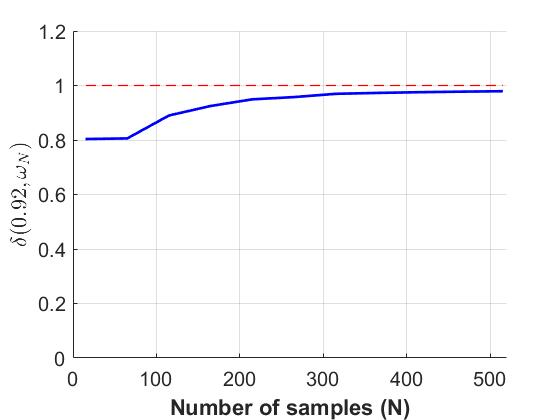
\includegraphics[scale=0.35]{delta1.jpg}

\caption{Evolution of $\delta$ along $N$.}
\label{fig:11}
\end{center}
\end{figure}

\begin{figure}
\begin{center}
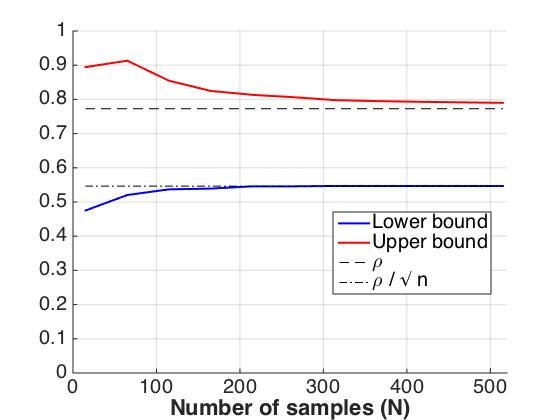
\includegraphics[scale=0.35]{bounds1.jpg}

\caption{Evolution of the bounds along $N$.}
\label{fig:21}
\end{center}
\end{figure}

We next test our algorithm on a $4$-dimensional system, with $5$ modes. We observe a slower convergence of $\delta$ as well as upper and lower bounds on $\rho$.
\textcolor{blue}{[to add plots here, but they are not super nice: we do not see the convergence to $1$ of $\delta$: even after $10 000$ points, $\delta$ is below $0.85$].}

Finally, we randomly generate $10,000$ cases with systems of dimension between $2$ and $7$, number of modes between $2$ and $5$, and size of samples $N$ between $30$ and $800$. We take $\beta = 0.92$ and we check if the upper bound computed by our techniques is greater than the actual JSR of the system. We get $xxx$ positive tests, out of $10,000$, which gives us a probability of $??$ of the correctness of the upper bound computed. Note that, this probability is significantly above the provided $\beta$. This is expected, since our techniques are based on worst-case analysis and thus conservative.



